\documentclass[a4paper,14pt]{extarticle}
\usepackage[labelformat=empty]{subfig}
\usepackage{float}
\usepackage{cmap}
\usepackage[T2A]{fontenc}
\usepackage[utf8x]{inputenc}
\usepackage[english, russian]{babel}
\usepackage{tikz}
\usetikzlibrary{positioning}

\usepackage{misccorr} % в заголовках появляется точка, но при ссылке на них ее нет
\usepackage{amssymb,amsfonts,amsmath,amsthm}  
\usepackage{indentfirst}
\usepackage[usenames,dvipsnames]{color} 
\usepackage[unicode,hidelinks]{hyperref}
% \hypersetup{%
%     pdfborder = {0 0 0}
% }
\usepackage{makecell,multirow} 
\usepackage{ulem}
\usepackage{graphicx,wrapfig} 
\graphicspath{{img/}}
\usepackage{geometry}
\geometry{left=3cm,right=1.5cm,top=2cm,bottom=2cm,bindingoffset=0cm,headheight=15pt}
\usepackage{fancyhdr} 
\linespread{1.5} 
\frenchspacing 
\renewcommand{\labelenumii}{\theenumii)} 
% \usepackage{caption}
%\documentclass[12pt]{article}
%\usepackage{ucs}
%\usepackage[left=20mm, top=20mm, right=10mm, bottom=20mm, nohead, nofoot]{geometry}
%\usepackage{graphicx}
%\graphicspath{{pictures/}}
%\DeclareGraphicsExtensions{.pdf,.png,.jpg}
%\usepackage[dvips]{graphicx}
%\usepackage[utf8x]{inputenc} 
%\usepackage[russian]{babel}  
%\usepackage{minted}
\title{\LaTeX}
\begin{document}
\begin{titlepage}
%\begin{spacing}{1.5}


  \begin{center}
    {\fontsize{ 12pt }{ 12pt } \selectfont \bf 
    МИНИСТЕРСТВО НАУКИ И ВЫСШЕГО ОБРАЗОВАНИЯ \\[-10pt] 
    РОССИЙСКОЙ ФЕДЕРАЦИИ}\\
    %\vspace{12pt}
    \begin{spacing}{}
      {\bf  Федеральное государственное автономное \\
      образовательное учреждение высшего образования \\
      <<Национальный исследовательский Нижегородский \\ 
      государственный университет им. Н.И. Лобачевского>>
      }
    \end{spacing}
    %\vspace{24pt}
    \begin{spacing}{}
      Радиофизический факультет\\
      %\vspace{20pt}
      Направление 03.03.03 «Радиофизика»\\
    Профиль «Фундаментальная радиофизика»\\
      \vspace{20pt}
      % ОТЧЕТ ПО $\ldots$ ПРАКТИКЕ
      ВЫПУСКНАЯ КВАЛИФИКАЦИОННАЯ РАБОТА БАКАЛАВРА\\
      \vspace{10pt}
      \textbf{\textsc{\Large
      Разработка автоматизированного метода отслеживания флуоресцентных областей при фотодинамической терапии
      }}
    \end{spacing}
    %\vspace{100pt}
    %\begin{equation}
    \end{center}
    \begin{aligned}
    &\text{ «К защите допущен»: }\quad
         &\text{}\\
        &\text{Руководитель практики:}\quad
         &\text{}\\
          &\text{д.ф.-м.н., профессор, зав. каф. общ. физики}\quad
          &\text{$\underline{\hspace{2cm}}$Бакунов М.И.\;\;}\\
          &\text{Научный руководитель:}\quad
         &\text{}\\
          &\text{к. ф.- м. н., зав. отд. рф. методов в мед. ИПФ РАН}\quad
          &\text{$\underline{\hspace{2cm}}$Турчин И.В.\;\;\;\;}\\
        &\text{Рецензент:}\quad
         &\text{}\\
          &\text{к.ф.-м.н., старший научный сотрудник ИПФ РАН}\quad
          &\text{$\underline{\hspace{2cm}}$Шилягин П.А.\;}\\
        &\text{Консультант по технике безопасности:}\quad
         &\text{}\\
          &\text{к.ф.–м.н., доцент }\quad
          &\text{$\underline{\hspace{2cm}}$Клёмина А.В.\; }\\
        &\text{Студент 4-го курса бакалавриата:}\quad &\text{$\underline{\hspace{2cm}}$Лебедев А.А.\;\;\;\,}
        \end{aligned}
      
    %\end{equation}
  %\end{center}
  \vfill
  \begin{center}
    Нижний Новгород
    \\
    2022
  \end{center}
%\end{spacing}
\end{titlepage}

\newpage

\tableofcontents

\newpage

\section{Введение}
Фотодинамическая терапия (ФДТ) - один из нехирургических способов лечения рака и предраковых состояний. Метод основан на введении в организм пациента поверхностно или внутривенно вещества - фотосенсибилизатора (ФС) (Рис. 1), его селективном накоплении и удерживании в области патологии (например, опухоли) и дальнейшем  облучении этой области светом определенной длины волны, соответствующей максимуму поглощения ФС или близкой к нему. 

\begin{center}
    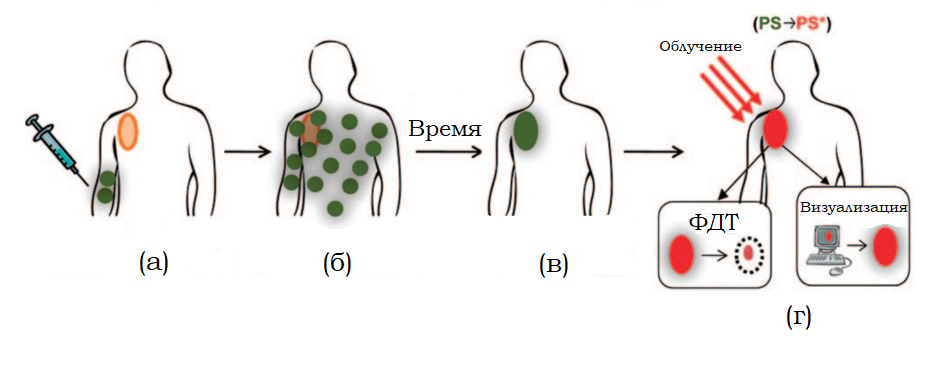
\includegraphics[scale = 0.7]{FDT.png}
    
    \textbf{Рис. 1.} Схема фотодинамической терапии [1]\\
    (а) - введение ФС,
    (б) - распространенеие ФС по организму,
    (в) - локализация ФС в измененных тканях,
    (г) - облучение опухоли светом определенной длины волны
\end{center}

При взаимодействии фотосенсибилизатора со светом в присутствии кислорода происходит фотохимическая реакция, в результате которой образуются активные формы кислорода, которые приводят к гибели клеток и микроорганизмов.
Наиболее распространенными ФС являются фотосенсибилизаторы с пиком поглощения в дальне-красной(>650 нм) и ближней ИК области спектра, где поглощение биоткани минимально и, соответственно, глубина проникновения света в ткани максимальна, что позволяет проводить ФДТ для опухолей, расположенных на глубине до нескольких миллиметров. Одним из таких ФС, широко распространненным в Российской Федерации, являются фотосенсибилизаторы хлоринового ряда с пиком поглощения 660 нм. Спектр поглощения ФС хлоринового ряда приведен на рисунке 2. 


\begin{center}
    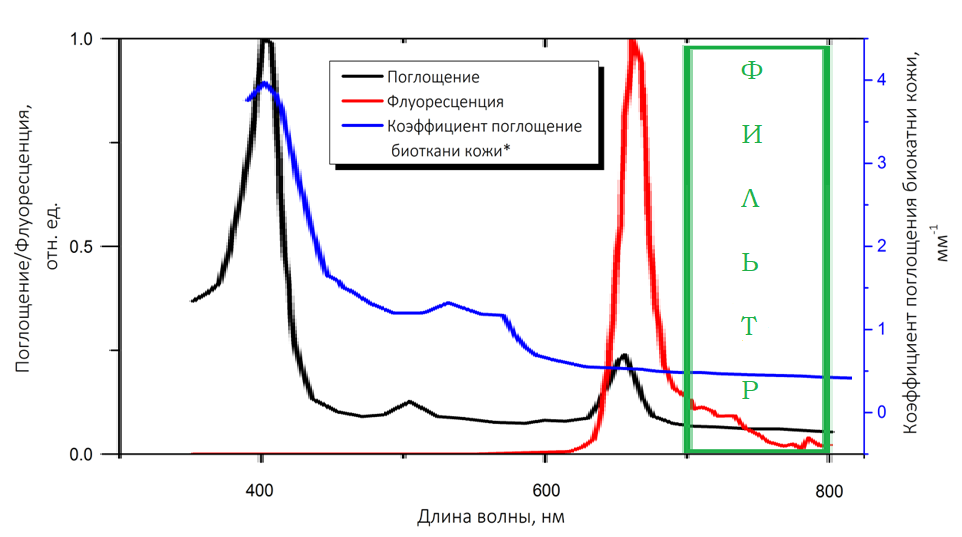
\includegraphics[scale = 0.6]{spektr.png}
    
    \textbf{Рис. 2.} Спектры поглощения (черная линия) и флуоресценции (красная линия) фотосенсибилизаторов хлоринового ряда. Синей линией обозначен спектр усредненного показателя поглощения биоткани. Зеленым прямоугольником обозначен спектр пропускания фильтра эмиссии
\end{center}


\begin{center}
    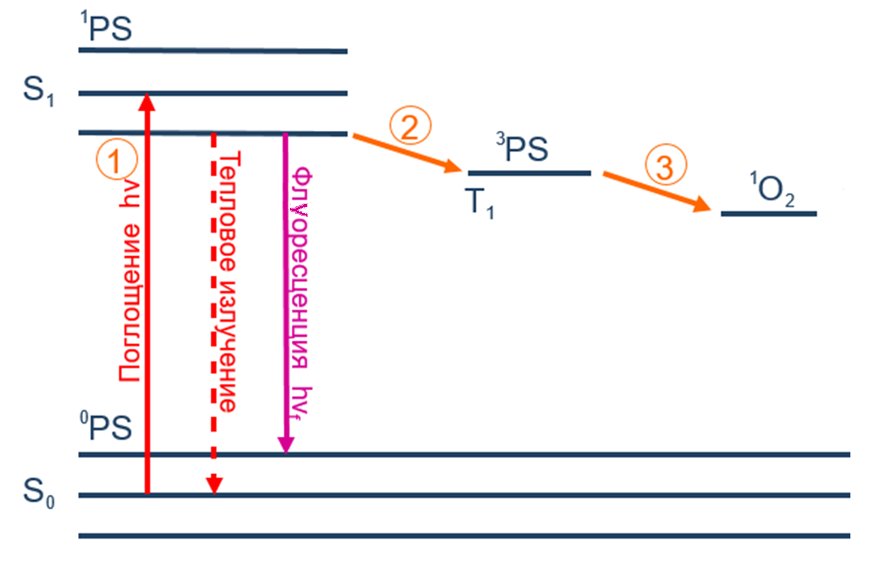
\includegraphics[scale = 0.6]{levels.png}
    
    \textbf{Рис. 3.} Структура энергетических уровней фотосенсибилизатора хлоринового ряда.
    $PS$ – фотосенсибилизатор,
    $_0PS$ – синглетное основное состояние,
    $_1PS$ – возбуждённое синглетное состояние,
    $_3PS$ – возбуждённое триплетное состояние,
    $h\nu$ – возбуждающее излучение,
    $h\nu_f$ – флуоресценция,
    $^1O_2$ – синглетный кислород.
\end{center}

На рисунке 3 изображена схема энергетических уровней фотосенсибилизатора хлоринового ряда - хлорина е-6. 

На схеме можно выделить несколько особых участков:
\begin{enumerate}
    \item $^0PS + h\nu \xrightarrow{} $ $^1PS $–поглощение фотона света определенной длины волны и энергетический переход фотосенсибилизатора в короткоживущее возбужденное синглетное состояние
    \item $^1PS \xrightarrow{} $ $^3PS $–переход фотосенсибилизатора в триплетное состояние
    \item $^3PS + O_2 \xrightarrow{} $ $^0PS +$ $ ^1O_2 $–передача энергии фотосенсибилизатора молекулярному кислороду, приводящая к возвращению фотосенсибилизатора в синглетное основное состояние и к появлению активного синглетного кислорода
\end{enumerate}

Как видно из рисунка 3, в ФС существуют излучательные переходы, что позволяет исследовать накопление и выведение из организма ФС методами флуоресцентной визуализации. В целом данные методы заключаются в облучении исследуемого участка ткани лазерным или светодиодным излучением, возбуждающим флуоресценцию, а регистрация эмиссии  флуоресценции осуществляется с помощью камер и фотодетекторов с оптическим фильтром, «отсекающим» возбуждающее излучение. [3] При этом для флуоресцентной визуализации используются гораздо более низкие плотности мощности, чем для процедуры ФДТ.
Помимо накопления и выведения ФС метод флуоресцентного имиджинга позволяет отслеживать фотовыгорание фотосенсибилизатора в процессе лазерного воздействия при ФДТ. Как показано в работах [1],[2],[3], степень выгорания ФС в процессе проведения терапии может являться критерием успешности ФДТ, заключающийся в минимизации рисков рецидивов. Динамика выгорания ФС может быть также использована для реализации обратной связи между врачом и пациентом, заключающейся в том, что при достижении определенного порога выгорания процедуру ФДТ необходимо остановить, чтобы, с одной стороны, снизить вероятность образования рецидивов, а с другой – минимизировать повреждение здоровых тканей. Таким образом, оптимальная доза облучения опухолевого узла может быть определена индивидуально в зависимости от оптических свойств области опухоли, степени ее кровоснабжения, присутствия кислорода в тканях и др. Однако к настоящему времени таких критериев, позволяющих индивидуально определять оптимальную дозу излучения, выработано не было из-за отсутствия систем количественного мониторинга выгорания ФС.
Для решения данной проблемы в Институте прикладной физики Российской Академии Наук(ИПФ РАН) был создан прибор - флуовизор, изображенный на рисунке 3а, позволяющий осуществлять флуоресцентную визуализацию фотосенсибилизатора, введенного в организм.


\begin{center}
    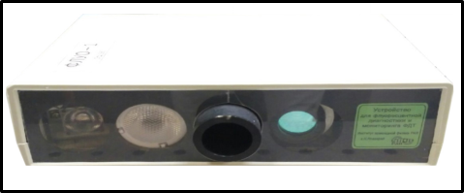
\includegraphics[scale = 0.6]{Fluo.png}
    
    (а)
    
\end{center}
\begin{center}
    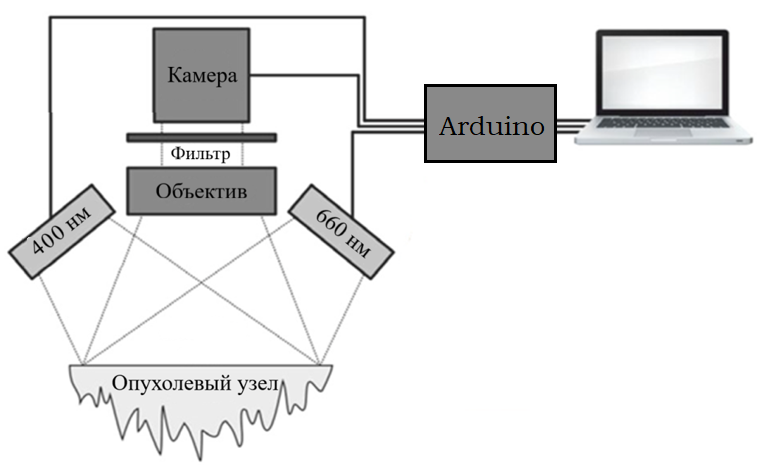
\includegraphics[scale = 0.7]{Fluo_shem.png}
    
    (б)
    
    \textbf{Рис. 3.} Внешний вид(а) и схема работы(б) прибора "Флуовизор"
\end{center}

Рисунок 3б иллюстрирует схему работы Флуовизора.
Опухолевый узел облучается светодиодами одной из возбуждающих длин волн 660 нм или 400 нм, соответствующих пикам поглощения ФС в красной и синей областях спектра (Рис. 2). Пространственное распределение интенсивности флуоресценции ФС регистрируется видеокамерой с применением интерференционного фильтра с полосой пропускания 700-800 нм. (Рис. 2). Также прибор облучает объект светодиодом на длине волны 740 нм, находящейся в спектре пропускания фильтра эмиссии, для получения изображения в обратно рассеянном свете. Кроме того,  CCD - камера регистрирует «темновой» (или «фоновый») кадр при выключенных светодиодах, который вычитается из кадров, полученных при облучении разными светодиодами для учета влияния фоновой засветки. Получение кадров с помощью цифровой камеры синхронизируются с точностью до нескольких микросекунд с включением/выключением светодиодов при помощи модуля Arduino, который в свою очередь соединен посредством USB порта с компьютером. Поступающие в память компьютера цифровые изображения визуализируются в специализированном приложении для ПК, реализованном на языке программирования Python. Скриншот интерфейса приложения приведен на рисунке 5.


\begin{center}
    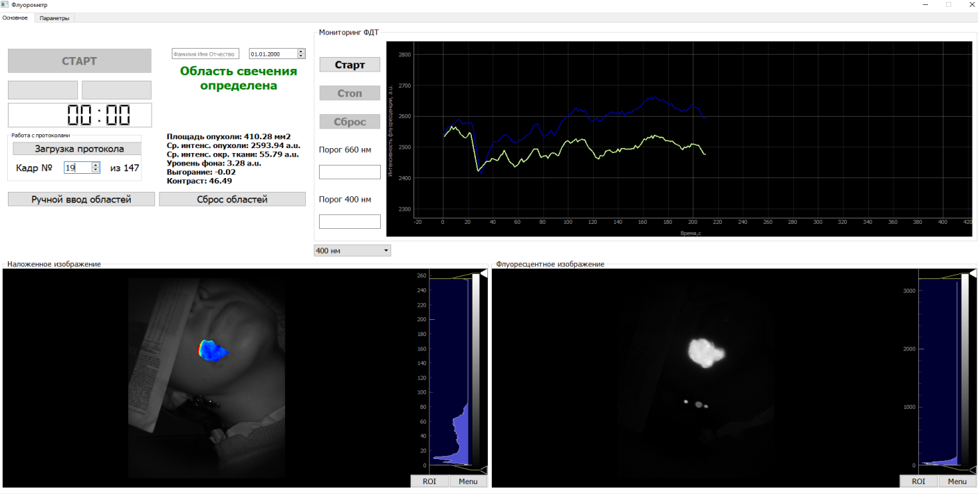
\includegraphics[scale = 0.8]{skrin.png}
    
    \textbf{Рис. 5.} Интерфейс ПО устройства Флуовизор
\end{center}

Прибор осуществляет визуализацию динамики выгорания фотосенсибилизатора в тканях пациента путем оценки динамики средней интенсивности его флуоресценции в опухолевом узле.
На данный момент флуовизор не способен вести слежение за флуоресцирующей областью, из-за чего обработку данных(кадров снятых флуовизором) приходится проводить вручную, размечая область на каждом из множества кадров.
Данную проблему решали сотрудники ИПФРАН, применяя детектирование флуоресцентной области при помощи обученного на это каскада Хаара. К сожалению, эксперименты не увенчались успехом из-за большого шумового фона, и точное детектирование реализовать не удалось.
 
В данной работе предлагается принципиально новый подход к решению данной проблемы - отслеживание или трекинг (от англ. track - следить) области. Идея заключается в том, что область опухолевого узла выделяется вручную только на первом кадре, а, далее она автоматически определяться на следующих изображениях при помощи алгоритма отслеживания. Для реализации данного подхода были разработаны несколько специализированных программ:


\begin{enumerate}
    \item Программа разметки изображений опухолевых узлов, описанная в Разделе 3. Данная программа необходима для ручной разметки положений опухолевых узлов. Разметка, осуществленная вручную для всех кадров, полученных в результате сеанса ФДТ, используется в качестве эталонной (“gold standard”) для последующей оценки эффективности работы автоматизированных трекеров. Кроме того, ручная разметка применяется для первого кадра сеанса ФДТ для реализации автоматизированного детектора. 
    \item Тестировочная программа для оценки эффективности работы алгоритмов. Для детектирования было выбрано несколько алгоритмов: Median Flow, TLD (Tracking-Modeling-Detection), MOSSE (Minimum Output Sum of Squared Error), CSRT (Channel and Spatial Reliability Tracker) , описанных в Разделе 2, наиболее подходящих для автоматизированного отслеживания опухолевого узла в процессе ФДТ.
    \item Программа для стандартизации полученных данных, принцип работы которой описан в Разделе 3. Выходные данные, полученные программами описанными в пунктах 1 и 2, были приведены к единому виду для проведения анализа. 
\end{enumerate}

\newpage 
\section{Алгоритмы отслеживания(трекинга), выбранные для анализа}

При анализе данных сеансов ФДТ, было выяснено, что флуоресцентная область смещается незначительно по сравнению с масштабом изображения. Данный факт позволяет включить в список исследуемых  алгоритмов трекинга методы, основанные на небольшом изменении оптического потока в серии изображений. Этот принцип лег в основу таких алгоритмов трекинга как Median Flow(раздел 2.2) и TLD(раздел 2.3).

Также в качестве особенностей серий изображений, следует отметить их схожесть друг с другом. Данный факт позволил включить в анализ алгоритмы, основанные на создании корреляционного фильтра. В работе рассматриваются трекеры MOSSE(раздел 2.1) и CSRT(раздел 2.4)     

\subsection{Трекер MOSSE}
\subsubsection{Отслеживание на основе корреляционного фильтра}

Трекеры на основе корреляционных фильтров моделируют внешний вид объектов, используя фильтр, обученный на примерах изображений. Область интереса изначально выбирается внутри прямоугольника на первом кадре.[5]

Цель отслеживается путем сопоставления фильтра с окном поиска в следующем кадре для определения местоположения, соответствующего максимальному значению выходных данных - корреляции. Далее выполняется оперативное обновление, на основе которого реализуется динамическое определение координат выбранной области.

Чтобы создать быстрый трекер, необходимо перейти из прямого пространства в Фурье при помощи БПФ(быстрое преобразование Фурье). 


Сначала вычисляется 2D-преобразование Фурье входного изображения: F = F(f) и фильтра: H = F(h). Теорема о свертке утверждает, что корреляция становится поэлементным умножением в области Фурье. Используя символ $\odot$  для явного обозначения поэлементного умножения и ∗ для обозначения комплексно-сопряженного элемента, корреляция принимает вид:

\begin{equation}
    G = F \odot H^*        
\end{equation}

Выходная функция G преобразуется обратно в пространственную область с использованием обратного БПФ. Сложность этих алгоритмов оценивается как $P \cdot log(P)$, где P - количество пикселей в окне отслеживания.

%В этом разделе мы обсудим компоненты трекеров на основе фильтров. В разделе 3.1 обсуждается предварительная обработка, выполняемая в окне отслеживания. Раздел 3.2 вводит Фильтры МОССА, которые являются улучшенным способом построения стабильного корреляционного фильтра из небольшого количества изображений. В разделе 3.3 показано, как регуляризация может быть использована для создания более стабильных фильтров UMACE и ASEF. В разделе 3.4 обсуждается простая стратегия, используемая для онлайн-обновления фильтров.

\subsubsection{Предварительная обработка}

Одна из проблем алгоритма свертки БПФ заключается в том, что изображение и фильтр сопоставляются с топологической структурой тора. Другими словами, он соединяет левый край изображения с правым краем, а верхний - с нижним.

Искусственное соединение границ изображения приводит к появлению разрыва на границе, который влияет на результат корреляции. Этот эффект уменьшается при выполнении предварительной обработки, которая заключается в следующем: 

\begin{enumerate}
    \item Значения пикселей нормализуются, чтобы иметь среднее значение в пределах от 0 до 1 и норму 1.
    \item Изображение умножается на окно косинуса, которое постепенно уменьшает значения пикселей вблизи края до нуля и создает больший акцент на центре области.
\end{enumerate}



\subsubsection{MOSSE Filters}

MOSSE(Minimum Output Sum of Squared Error) - это алгоритм для создания ASEF(Average of Synthetic Exact Filters)-подобных фильтров из меньшего количества обучающих изображений. Для начала ему необходим набор обучающих изображений $f_i$ и обучающих выходных данных $g_i$. Как правило, $f_i$ может принимать любую форму. В этом случае $g_i$ определяется как, 2D пик гауссовой формы($\sigma$ = 2.0), центрированный на цели в обучающем изображении $f_i$. Обучение проводится в области Фурье, чтобы воспользоваться преимуществами простой поэлементной взаимосвязи между входными и выходными данными. 

%Как и в предыдущем разделе, мы определяем переменные верхнего регистра Fi, Gi и фильтр H для быть преобразованием Фурье их аналогов в нижнем регистре.
\begin{equation}
    H_i^* = \frac{G_i}{F_i}
\end{equation}
где деление выполняется поэлементно.


Чтобы найти фильтр, который сопоставляет входные данные обучения с желаемыми выходными данными, MOSSE находит значение H, которое минимизирует сумму квадратов ошибок между фактическим и желаемым результатом свертки.

Эта задача минимизации имеет вид:

\begin{equation}
    \min_{H^*}\sum_i |F_i \odot H^* - G_i|^2
\end{equation}

%Идея минимизации суммы квадратов ошибок (SSE) над выводом нет ничего нового. Фактически, задача оптимизации в уравнении 3 почти идентична задачам оптимизации, представленным в [10] и [12]. Разница в том, что в этих работах предполагалось, что цель всегда тщательно центрировалась в fi и что выходные данные (gi) были фиксированными для всего обучающего набора, тогда как настройка каждого gi является фундаментальной идеей ASEF и MOSSE. 

Идея минмизации суммы квадратов ошибок(SSE) была выдвинута еще до создания трекера MOSSE, но в работах ученых того времени предполагалось, что цель всегда явно локализована в центре $f_i$. 

В задаче отслеживания цель не всегда центрирована, и пик в $g_i$ перемещается, чтобы следовать за целью в $f_i$. В более общем случае $g_i$ может иметь любую форму. Например, в $f_i$ содержится несколько целевых значений, а $g_i$ имеет несколько соответствующих пиков. 


Рассмотрим решение задачи оптимизации (3). Отметим, что каждый элемент $H$ (индексированный $\omega$ и $\nu$)
может быть вычислен независимо, поскольку все операции в области Фурье выполняются поэлементно. Это включает в себя переписывание функции в терминах как $H_\omega_\nu$, так и $H^*_{\omega\nu}$. Тогда частная производная по $H^*_{\omega\nu}$ становится равной нулю, при этом $H_\omega_\nu$ рассматривается как независимая переменная.


\begin{equation}
     \frac{\partial}{\partial H^*_{\omega\nu}}\sum_i |F_{i\omega\nu} \odot H^*_{\omega\nu} - G_{i\omega\nu}|^2 = 0
\end{equation}

\begin{equation}
     \frac{\partial}{\partial H^*_{\omega\nu}}\sum_i (F_{i\omega\nu} \odot H^*_{\omega\nu} - G_{i\omega\nu})\cdot (F_{i\omega\nu} \odot H^*_{\omega\nu} - G_{i\omega\nu})^* = 0
\end{equation}

\begin{equation}
     \frac{\partial}{\partial H^*_{\omega\nu}}\sum_i \Big[(F_{i\omega\nu}H^*_{\omega\nu})(F_{i\omega\nu}H^*_{\omega\nu})^* - (F_{i\omega\nu}H^*_{\omega\nu})G^*_{i\omega\nu} - G_{i\omega\nu}(F_{i\omega\nu}H^*_{\omega\nu})^* + G_{i\omega\nu}G^*_{i\omega\nu}\Big] = 0
\end{equation}

\begin{equation}
     \frac{\partial}{\partial H^*_{\omega\nu}}\sum_i \Big[F_{i\omega\nu}H^*_{\omega\nu}F_{i\omega\nu}^*H_{\omega\nu} - F_{i\omega\nu}H^*_{\omega\nu}G^*_{i\omega\nu} - G_{i\omega\nu}F_{i\omega\nu}^*H_{\omega\nu} + G_{i\omega\nu}G^*_{i\omega\nu}\Big] = 0
\end{equation}

\begin{equation}
    \sum_i \Big[F_{i\omega\nu}F^*_{i\omega\nu}H_{i\omega\nu} - F_{i\omega\nu}G^*_{i\omega\nu}\Big]= 0
\end{equation}

\begin{equation}
    H_{\omega\nu} = \frac{\sum_i G^*_{i\omega\nu} \odot F^*_{i\omega\nu}}{\sum_i F_{i\omega\nu} \odot F_{i\omega\nu}}
\end{equation}

Путем решения для $H^*$ найдено выражение для фильтра MOSSE:

\begin{equation}
    H^* = \frac{\sum_i G_i \odot F_i^*}{\sum_i F_i \odot F_i^*}
\end{equation}

Компоненты уравнения 10 имеют интересную интерпретацию. Числитель - это корреляция между входным сигналом и желаемым
выходом, а знаменатель - энергетический спектр
входного сигнала.
%Из уравнения 5 мы можем легко показать, что UMACE является частным случаем MOSSE. UMACE определяется как H∗ = D−1m∗, где m - вектор, содержащий БПФ средних центрированных обрезанных обучающих изображений, а D - диагональная матрица, содержащая средний энергетический спектр обучающих изображений [18]. Поскольку D - диагональная матрица, умножение на ее обратную величину по существу выполняет

Таким образом в нашем случае получаем корреляцию в виде: 

\begin{equation}
    G = F \odot \frac{\sum_i G_i \odot F_i^*}{\sum_i F_i \odot F_i^*}
\end{equation}




\subsection{Трекер Median Flow}
\subsubsection{Метод Лукаса-Канаде}

%\begin{enumerate}
%    \item $I(x,y,t)$ - оптический поток
%    \item $u_x, u_y$ - координаты вектора смещения
%    \item $t$ - номер кадра
%\end{enumerate}

В основе алгоритма лежит положение о том, что пиксели переходят из кадра в кадр без изменений. Математически это суждение можно описать как:

\begin{equation}
    I(x,y,t) = I(x+u_x,y+u_y,t+1),
\end{equation}
где $I(x,y,t)$ - оптический поток, $t$ - номер кадра

Из предположения о малом изменении оптического потока между кадрами, разложим функцию $I(x,y)$ в ряд Тейлора до линейного члена включительно.[6]

\begin{equation}
    I(x+u_x,y+u_y,t) = I(x,y,t) + \vec u \cdot \nabla I(x,y,t),
\end{equation}
где $\vec{u} = (u_x, u_y)$ - вектор смещения

В соответствии с (12):

\begin{equation}
    I(x,y,t+1) = I(x,y,t) + \vec u \cdot \nabla I(x,y,t)  
\end{equation}

Заметим, что $I(x,y,t)$ - дискретная функция времени. Производную $I^'_t$ введем как $I(x,y,t)-I(x,y,t+1)$

\begin{equation}
    \frac{\partial I(x,y,t)}{\partial t} + \vec u \cdot \nabla I(x,y,t) = 0
\end{equation}

\begin{equation}
    \frac{\partial I(x,y,t)}{\partial t} + u_x \cdot \frac{\partial I(x,y,t)}{\partial x} + u_y \cdot \frac{\partial I(x,y,t)}{\partial y} = 0
\end{equation}

Для дальнейшего анализа понадобится еще одно приближение. Предположим, что участок изображения движется как единое целое, тогда для описания смещения необходимо одно уравнение. Но если область интереса представляет из себя, например, квадрат, размером 5x5, мы имеем 25 особых точек(пикселей). В этом случае вместо одного мы получим 25 уравнений. Очевидно, что в общем случае система не имеет решения, поэтому будем искать такие, которые минимизируют ошибку.

\begin{equation}
    E(u_x,u_y) = \sum_{i,j} g(x_i,y_i)\Big[\frac{\partial I(x,y,t)}{\partial t} + u_x \cdot \frac{\partial I(x,y,t)}{\partial x} + u_y \cdot \frac{\partial I(x,y,t)}{\partial y}\Big]^2
\end{equation}
$g(x_i,y_i)$ - функция, определяющая весовые коэффициенты пикселей. Чаще всго используются двумерная гауссина, усиливающая вес пикселей, находящихся в центре. 

Для нахождения миннимума функции ошибок $E(u_x,u_y)$ воспользуемся методом наименьших квадратов. Найдем частные производные E по $u_x$ и $u_y$.
\begin{equation}
    \frac{\partial E}{\partial u_x} = 2\sum_{i,j} g(x_i,y_i)\Big[\frac{\partial I(x_i,y_i,t)}{\partial t} + u_x \frac{\partial I(x_i,y_i,t)}{\partial x} + u_y \frac{\partial I(x_i,y_i,t)}{\partial y}\Big] \frac{\partial I(x_i,y_i,t)}{\partial x}= 
\end{equation}

\begin{displaymath}
    =2\sum_{i,j}g(x_i,y_i)\Big[u_x\Big(\frac{\partial I(x_i,y_i,t)}{\partial x}\Big)^2 + u_y\frac{\partial I(x_i,y_i,t)}{\partial y}\frac{\partial I(x_i,y_i,t)}{\partial x} + \frac{\partial I(x_i,y_i,t)}{\partial t} \cdot
\end{displaymath}

\begin{displaymath}
    \cdot \frac{\partial I(x_i,y_i,t)}{\partial x}\Big]
\end{displaymath}




\begin{equation}
    \frac{\partial E}{\partial u_y} = 2\sum_{i,j} g(x_i,y_i)\Big[\frac{\partial I(x_i,y_i,t)}{\partial t} + u_x \frac{\partial I(x_i,y_i,t)}{\partial x} + u_y \frac{\partial I(x_i,y_i,t)}{\partial y}\Big] \frac{\partial I(x_i,y_i,t)}{\partial y}= 
\end{equation}

\begin{displaymath}
    =2\sum_{i,j}g(x_i,y_i)\Big[u_y\Big(\frac{\partial I(x_i,y_i,t)}{\partial y}\Big)^2 + u_x\frac{\partial I(x_i,y_i,t)}{\partial x}\frac{\partial I(x_i,y_i,t)}{\partial y} + \frac{\partial I(x_i,y_i,t)}{\partial t} \cdot
\end{displaymath}

\begin{displaymath}
    \cdot \frac{\partial I(x_i,y_i,t)}{\partial y}\Big]
\end{displaymath}

Запишем полученные уравнения, положив частные производные равными нулю.

\begin{displaymath}
   \frac{\partial E(u_x,u_y)}{\partial u_x} = \sum_{i,j}g(x_i,y_j)\Big[ u_x \Big( \frac{\partial I}{\partial x}\Big)^2 + u_y \frac{\partial I}{\partial y} \frac{\partial I}{\partial x} + \frac{\partial I}{\partial t}\frac{\partial I}{\partial x}\Big] = 0
\end{displaymath}

\begin{displaymath}
   \frac{\partial E(u_x,u_y)}{\partial u_y} = \sum_{i,j}g(x_i,y_j)\Big[ u_y \Big( \frac{\partial I}{\partial y}\Big)^2 + u_x \frac{\partial I}{\partial x} \frac{\partial I}{\partial y} + \frac{\partial I}{\partial t}\frac{\partial I}{\partial y}\Big] = 0
\end{displaymath}
Перепишем уравнения в матричной форме: 
\begin{equation}
    M\cdot \vec u = \vec b
\end{equation}
M = \begin{vmatrix}
    \sum_{i,j}g(x_i,y_i)\Big( \frac{\partial I}{\partial x}\Big)^2 & \sum_{i,j}g(x_i,y_i)\Big( \frac{\partial I}{\partial x}\frac{\partial I}{\partial y}\Big) \\
    \sum_{i,j}g(x_i,y_i)\Big( \frac{\partial I}{\partial x}\frac{\partial I}{\partial y}\Big) & \sum_{i,j}g(x_i,y_i)\Big( \frac{\partial I}{\partial x}\Big)^2
\end{vmatrix}
\bigskip \\
$\vec b = -$ \begin{vmatrix}
\sum_{i,j}g(x_i,y_i)\Big( \frac{\partial I}{\partial t}\frac{\partial I}{\partial x}\Big)\\
\sum_{i,j}g(x_i,y_i)\Big( \frac{\partial I}{\partial t}\frac{\partial I}{\partial y}\Big)
\end{vmatrix}
\bigskip \\
$\vec u = $ \begin{vmatrix}
u_x\\u_y
\end{vmatrix}

Соотношения (20) является уравнением перемещения окрестности точки (x,y). Отсюда несложно выразить вектор $\vec u$.

\begin{equation}
    \vec u = M^{-1} \cdot \vec b
\end{equation}

Но в реальных системах соотношение (20) не выполняется точно, поэтому задача алгоритма Лукаса-Канаде - это вариационная задача минимизации ошибки.

\begin{equation}
    \min_i \Big[ M_i \cdot \vec u_i - \vec b_i\Big]
\end{equation}




\subsubsection{Median-Flow}
Принцип работы трекера median-flow почти полностью описывается алгоритмом Лукаса-Канаде. На вход трекер получает пямоугольный участок изображения, который разбивается на небольшие части квадратной формы. Каждая из этих частей обрабатывается методом Лукаса - Канаде. В итоге имеется набор координат векторов смещения. Из массива абсцисс и массива ординат берутся медианные значения, из которых составляется вектор перемещения. Далее из списка координат точек исходного изображения и прогнозируемого берутся всевозможные пары точек. Между ними измеряется расстояние и находится отношение прогнозируемой длины отрезка к имеющейся на предыдущем кадре. Для более устойчивого выбора одного значения из всех также используется медианный метод. Данное число показывает изменение размера объекта в результате эволюции.


\subsection{Трекер TLD}

Рассмотренные выше алгоритмы отличаются от рассматриваемых далее авторским подходом к трекингу. Трекер TLD(Tracking-Modeling-Detection) основан на комбинации и связи элементов, указанных на рисунке 6.[8]

\begin{center}

\begin{tikzpicture}[
roundnode/.style={circle, draw=black!80, fill=white!5, very thick, minimum size=40mm},
squarednode/.style={rectangle, draw=red!60, fill=red!5, very thick, minimum size=10mm},
centernode/.style={rectangle, draw=white!60, fill=white!5, very thick, minimum size=10mm},
]
%Nodes
\node[centernode]        (maintopic)                            {};
\node[roundnode]        (uppercircle)       [above=of maintopic] {Обучение};
\node[roundnode]      (rightcircle)       [right=of maintopic] {Детектирование};
\node[roundnode]        (leftcircle)       [left=of maintopic] {Трекинг};

%Lines
\draw[->] (rightcircle.north) .. controls  + (up:7mm) and + (right:7mm)  .. (uppercircle.east);
\draw[->] (rightcircle.south) .. controls +(down:20mm) and +(down: 20mm) .. (leftcircle.south);
\draw[->] (leftcircle.north) .. controls  + (up:7mm) and + (left:7mm)  .. (uppercircle.west);
\draw[->] (uppercircle.south) .. controls  + (up:-7mm) and + (left:7mm)  .. (rightcircle.west);
\filldraw[black] (-2.5,-4) node[anchor=west]{Повторное обнаружение};
\filldraw[black] (-1.7,0) node[anchor=west]{Обучающие};
\filldraw[black] (-1.3,-0.5) node[anchor=west]{данные};
\filldraw[black] (-6.5,3) node[anchor=west]{Фрагменты};
\filldraw[black] (-6.5,2.5) node[anchor=west]{траектории};
\filldraw[black] (3.5,3) node[anchor=west]{Обнаружение};
%\filldraw[black] (0,0) circle (2pt) node[anchor=west]{Intersection point};
\end{tikzpicture}

\textbf{Рис.6.}Схема самообучающегося алгоритма трекинга
\end{center}

В основе трекера TLD положен алгоритм Лукаса-Канаде, описанный в разделе 2.2.1 с дополнительным модулем обучения.
\subsubsection{Детектор}
Детектор — это алгоритм, позволяющий найти заданный объект на изображении. Стратегия детектора, используемого в алгоритме TLD — стратегия сканирующего окна. Входное изображение сканируется окном и для каждого подизображения бинарный классификатор решает присутствует ли там объект или нет. Классификатор состоит из набора характеристик. По каждой происходит сравнение, подходит ли подизображение под характеристику или нет. Конечный результат вычисляется средним ответом. Если подизображение классифицируется положительно более чем 50 процентами характеристик, то классификатор даёт положительный ответ. В противном случае - отрицательный.

\subsubsection{Обучение}
Алгоритм является самообучающимся, используя для обучения
непомеченные данные. В качестве данных о положении объекта выступают результаты работы трекера. В случае, если расстояние между положением, указанным детектором близко к положению, указанным трекером, то результат работы детектора оценивается как положительный. В противном случае как отрицательный. 

%Модель в алгоритме TLD представляется в виде рандомизированного леса. Обучение происходит путём двух событий: расширяющего (при определении патча как положительного) и урезающего (при определении патча как отрицательного). Расширение модели необходимо для добавления новых правильных возможных состояний модели, и происходит добавлением и расширением веток. Урезание модели необходимо для удаления неверных образцов, и происходит путём удаления веток из леса.
\subsection{Трекер CSRT}
Алгоритм CSRT(Channel and Spatial Reliability Tracker) основан на процедуре DCF(Discriminative Correlation Filter). Метод повышает точность DCF за счет добавления карт пространственной надежности. Данная модификация позволяет корректировать полученный корреляционный фильтр при помощи серии неразмеченных данных. Алгоритм создает фильтр по первому изображению, которое необходимо разметить собственноручно, а затем модернизирует его при помощи поступающих новых данных.[7] Принципиальная схема работы представлена на рисунке 6.






























\newpage
\section{Разработка программы разметки}
Для тестирования разрабатываемого алгоритма трекинга в ИПФРАН были предоставлены базы данных изображений, полученных во время сеансов фотодинамической терапии в клинике при лечении онкологических заболеваний. База данных содержит в себе 5 сеансов ФДТ, каждый из которых включает в себя около 80 флуоресцентных изображений опухолевых узлов. 


Эталонная разметка положений опухолевого узла на этих кадрах может быть получена вручную. Для этого была разработана специализированная программа предобработки и разметки исходных данных. 


Так как исходные изображения поступили в формате .tiff, а используемые в дальнейшем инструменты такой тип данных не поддерживают, все изображения были переведены в .jpg при помощи программы перекодировки, реализованной на языке программирования Python. 


Для получения эталонных данных разметки на языке программирования Python был реализован следующий алгоритм:


\begin{enumerate}
    \item Разметить покадрово серию данных при помощи выделения на изображениях области интереса(опухолевого узла).
    \item Создание бинарной маски, которая выделяет область опухолевого узла значениями пикселей внутри, равными 255, значения пикселей вне данной области примет равными 0.
    \item Выделение опухолевого узла, путем умножения исходного изображения и маски.
    \item Создание структурированной области, путем обрезки данного изображения по границе опухолевого узла прямоугольной областью.
\end{enumerate}

В результате работы алгоритма в памяти компьютера сохраняются структурированные данные в виде опухолевых узлов, размеченных собственноручно пользователем. 

На рисунке 7а приведен скриншот работы программы разметки, где белым цветом обозначена область, заданная пользователем. Полученный в результате выделения на рисунке 7а, и, обработанный программой разметки, опухолевый узел изображен на рисунке 7б.


\begin{center}
    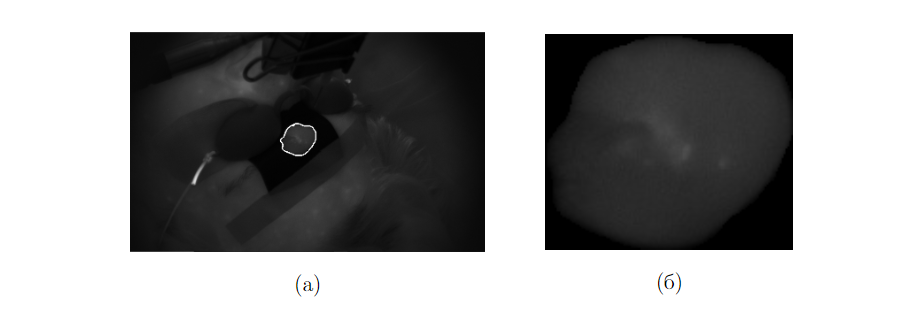
\includegraphics[scale = 0.85]{ab.PNG}
    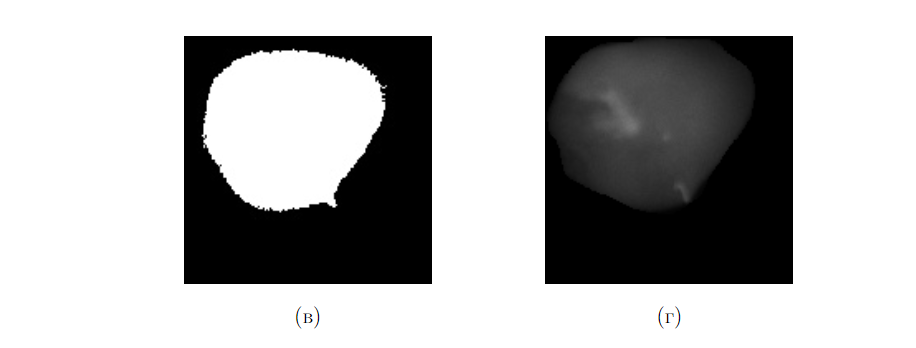
\includegraphics[scale = 0.85]{vg.PNG}
    \textbf{Рис.7.}(а)Скриншот работы программы на исходном изображении в разрешении .jpg; (б)Пример выходных данных из алгоритма разметки (в)Пример бинаризованной по среднему значению интенсивности маски; (г)Пример выходных данных из алгоритма разметки 
\end{center}

В результате работы программы, были получены базы данных структурированных опухолевых узлов, одна из которых приведена на рисунке 8а. Для удаления с изображений опухолевых узлов шумового фона, была создана бинарная маска по среднему значению интенсивности. Изображение полученной маски приведено на рисунке 7а. Полученная маска матрично умножалась на исходное изображение. Результат умножения приведен на рисунке 7б. Выходное изображение можно полностью считать изолированным от шумов.



\begin{figure}[p]
\begin{minipage}[p]{0.49\linewidth}
\center{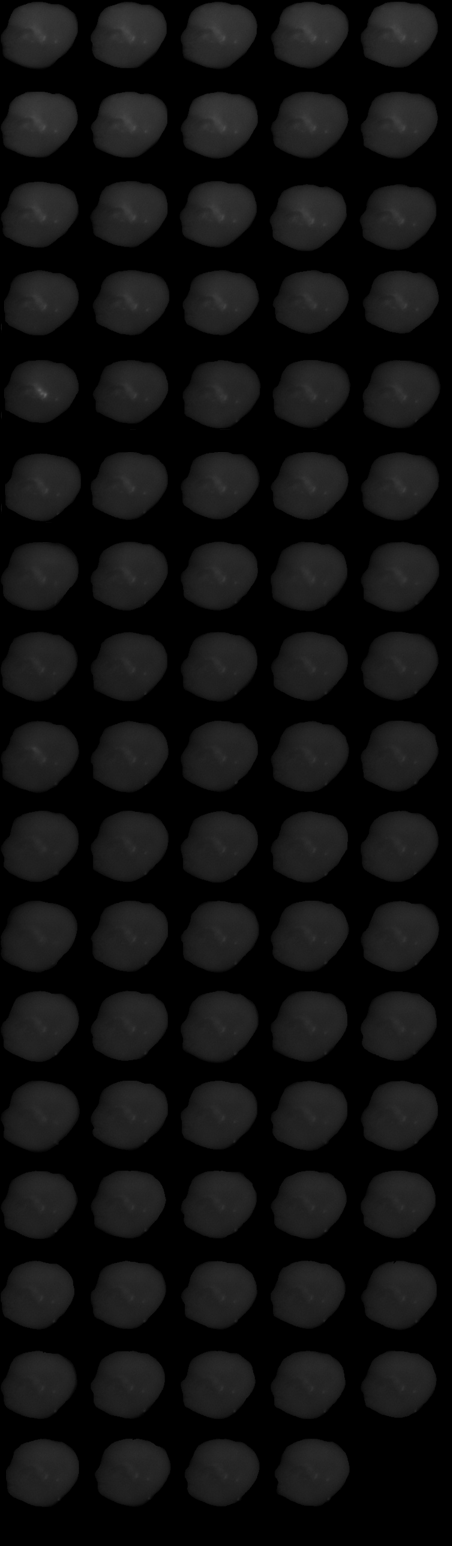
\includegraphics[width=0.8\linewidth]{all_masks.png} \\ (а)}
\end{minipage}
\hfill
\begin{minipage}[h]{0.49\linewidth}
\center{\includegraphics[width=0.85\linewidth]{models/all_masks_csrt.png} \\ (б)}
\end{minipage}
\begin{center}
   \textbf{Рис. 8.} База вырезанных опухолевых узлов одного из сеансов фотодинамической терапии, полученная (а)-вручную, (б)-алгоритмом CSRT 
\end{center}
\label{ris:image1}
\end{figure}






После структуризации данных и удаления шумов, была построена зависимость средней интенсивности флуоресценции опухолевого узла от времени после начала фотодинамической терапии, которая приведена на рисунке 9. Значение средней интенсивности вычислялось при помощи усреднения интенсивностей всех пикселей опухолевого узла. По оси ординат отложена нормированная по первому кадру безразмерное значение средней интенсивности флуоресценции. Сеанс лазерного воздействия периодически прерывался для работы Флуовизора – регистрации и записи флуоресцентных изображений. Таким образом, весь сеанс ФДТ состоял из кратковременных сеансов. Символами $h\nu$ на рисунке 9 отмечены начала этих кратковременных сеансов лазерного воздействия.  

Стоит заметить монотонное убывание средней интенсивности в процессе лазерного воздействия, что можно связать с фотобличинком (фотовыгоранием) ФС, а также его разрушением в результате образования активных форм кислорода. Минимуму данной зависимости соответствует окончание лазерного воздействия и, соответственно, максимальная доза лазерного излучения, полученная тканью. 

Также на рисунке 9 отмечена область, снятая после окончания ФДТ. Быстрое возрастание интенсивности флуоресценции опухолевго узла соответствует, по-видимому, притоку в измененные ткани нового фотосенсибилизатора, циркулирующего в организме, с кровью.







%\begin{center}
%    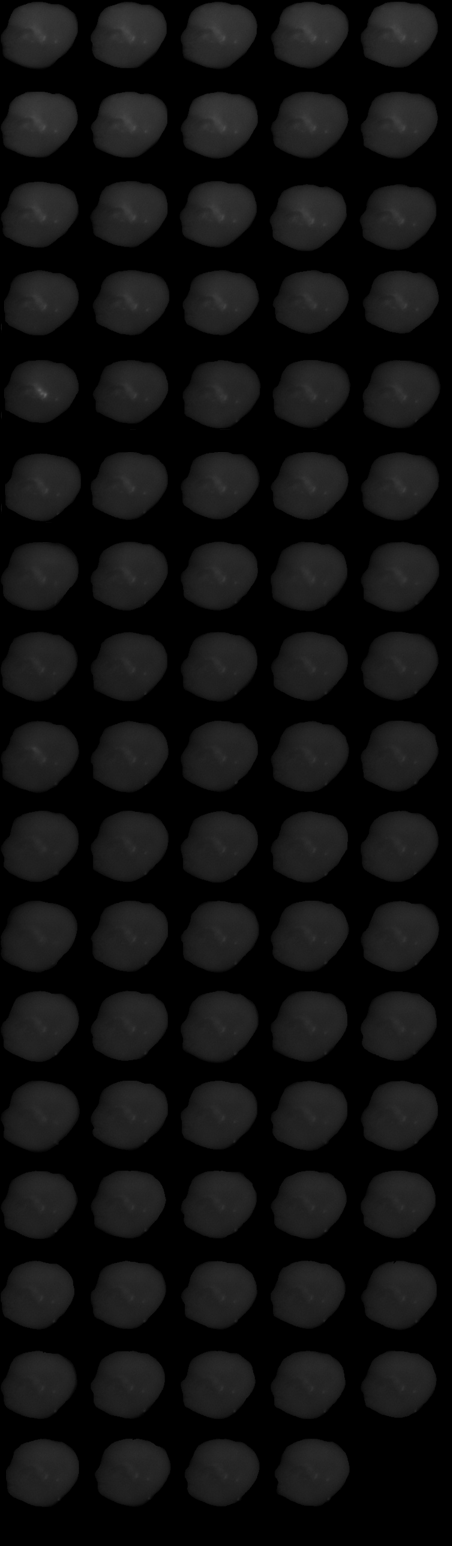
\includegraphics[scale = 0.7]{all_masks.png}
    
%    \textbf{Рис. 8.} База вырезанных опухолевых узлов одного из сеансов фотодинамической терапии, полученная вручную
%\end{center}








\begin{center}
    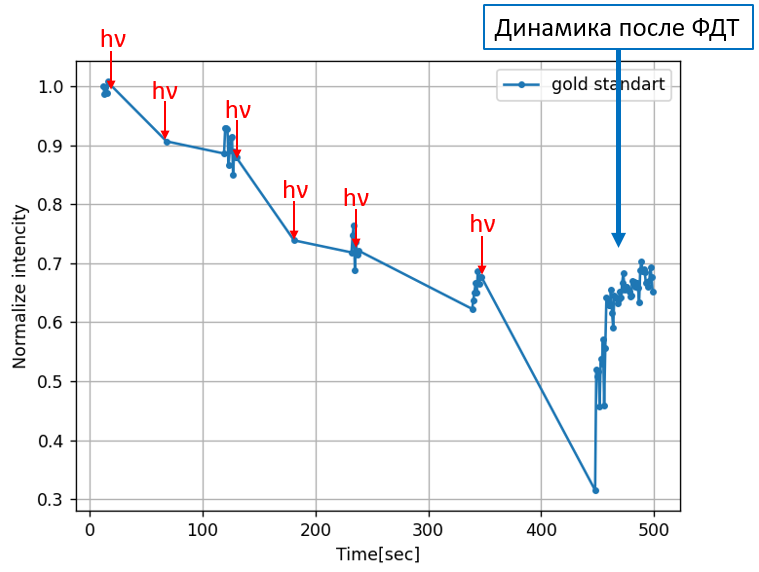
\includegraphics[scale = 0.9]{It.PNG}
    
    \textbf{Рис. 9.} Зависимость интенсивности флуоресценции от времени с начала ФДТ, полученная в результате ручной разметки флуоресцентных изображений  
\end{center}



\newpage 
\section{Разработка программы тестирования алгоритмов трекинга}
Для тестирования алгоритмов трекинга, описанных в Разделе 2, была создана тестировочная программа, которая способна получать и сохранять в память компьютера данные в том же формате, что были получены при ручной разметке. Для этого был реализован трекинг прямоугольной области, выбранной на первом изображении каждой серии и сохранение данных в память компьютера для дальнейшей обработки.


Полученная в результате работы программы база данных, приведена на рисунке 8б. 

Пример полученной в результате работы программы с алгоритмом CSRT базы данных, приведена на рисунке 8б.
Из данного рисунка видно, что размеры прямоугольника постоянно меняются. Это связано с особенностью методов отслеживания, заключающейся в том, что на каждом шаге работы алгоритма помимо определения координат области, он проверяет изменение размера объекта, что может приводить к небольшому изменению размеров области. Подобную картину можно наблюдать при анализе выходных данных каждого трекера.
Изображения, полученные тестировочной программой также прошли обработку, аналогичную описанной в разделе 3: были созданы бинарные маски, найдены интенсивности опухолевых узлов и построена зависимость нормированной интенсивности флуоресценции от времени после начала ФДТ, которая приведена на рисунке 10. Стоит отметить, что на рисунке 10 практически полностью перекрылась кривая "gold standart". 



\begin{center}
    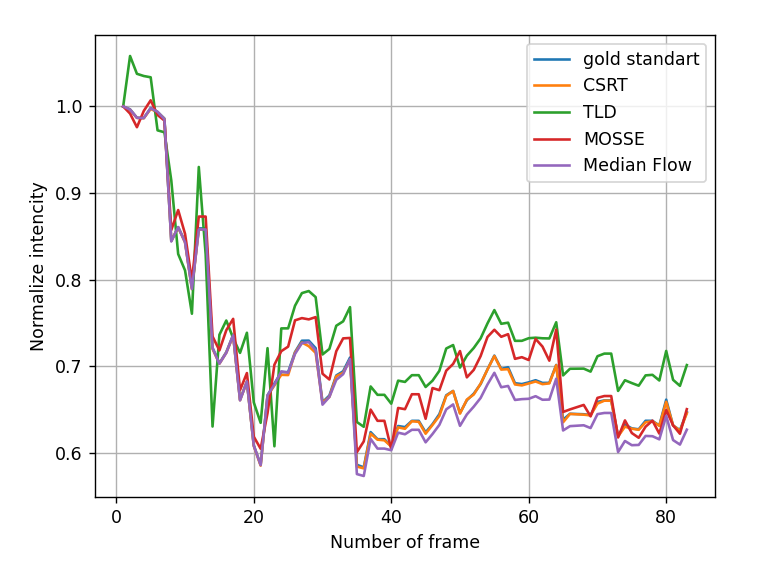
\includegraphics[scale = 0.9]{int_all.PNG}
    
    \textbf{Рис. 10.} Зависимость интенсивности флуоресценции от номера кадра(данные полученные алгоритмами трекинга)
\end{center}

\newpage
\section{Анализ полученных данных}
Чтобы сделать вывод о том, какой алгоритм трекинга оказался лучшим, была построена зависимость, отклонения интенсивности флуоресценции опухолевого узла от номера кадра, изображенная на рисунке 11. Так же была составлена сравнительная таблица 1.
В качестве критериев оценки эффективности работы алгоритмов были выбраны следующие критерии:


\begin{enumerate}
    \item СКО - среднеквадратичное отклонение от эталонной разметки
    \item МО - максимальное отклонение от эталонной разметки
    \item ССКО - среднее СКО по пяти сеансам ФДТ
    \item СМО - среднее МО по пяти сеансам ФДТ
    \item ММО - максимальное МО из пяти сеансов ФДТ
\end{enumerate}






\begin{center}
    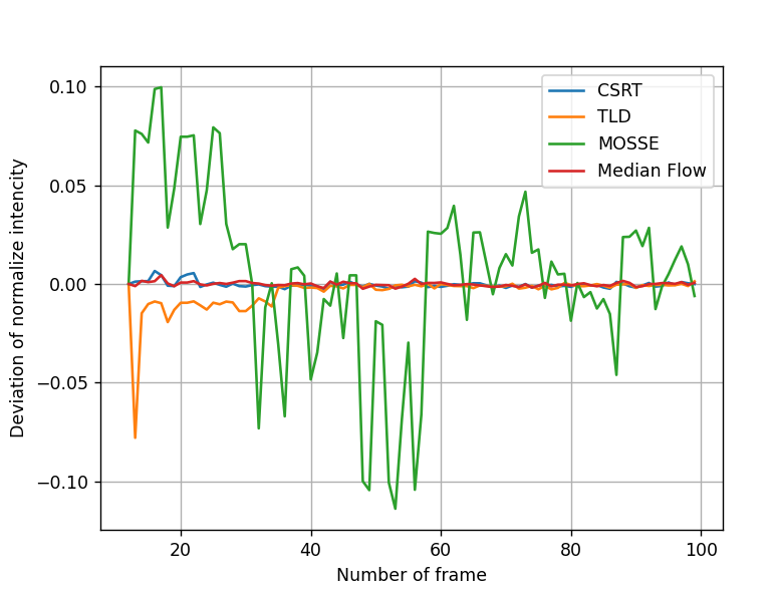
\includegraphics[scale = 0.8]{delta.png}
    
    \textbf{Рис. 11.} Зависимость отклонения нормированной интенсивности флуоресценции опухоли от номера кадра при использовании различных алгоритмов трекинга от значений, полученной при ручной разметке 
\end{center}

В результате анализа полученных данных по критериям ССКО, СМО и ММО, минимальные погрешности показали алгоритмы CSRT и Median Flow. Однако по скорости обработки данных (Таблица 1, "Скорость, FPS"), алгоритм CSRT уступает Median Flow почти в 7 раз, что говорит о том, что оптимальным для отслеживания флуоресцентных областей можно считать алгоритм Median Flow.    


\begin{center}
    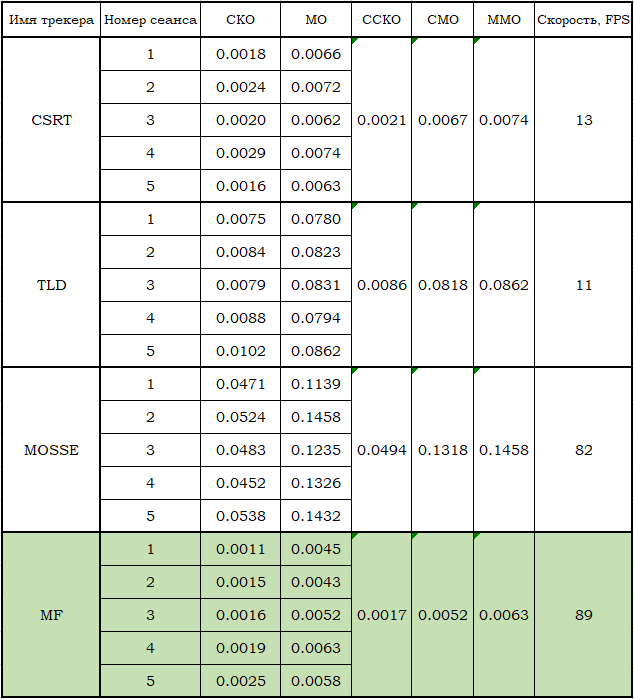
\includegraphics[scale = 1.2]{tab.png}
    
    
    \textbf{Табл. 1.} Сравнительная таблица разных алгоритмов трекинга
\end{center}



\newpage
\section{Заключение}
Данная работа направлена на разработку метода отслеживания флуоресцентных областей при мониторинге фотодинамической терапии (ФДТ). В результате была создана программа разметки изображений, полученных при сеансах фотодинамической терапии, необходимой для создания эталонных данных о положении опухолевого узла в процессе ФДТ. Для осуществления автоматизированного слежения за областью опухоли предложен подход трекинга выбранной на первом кадре области. В качестве алгоритмов трекинга были выбраны MOSSE, Median Flow, TLD, CSRT алгоритмы. Для их анализа была создана программа тестировки, благодаря которой были собраны данные работы алогритмов трекинга. Для определения лучшего алгоритма предложено использовать критерии СКО(среднеквадратичное отклонение), МО(максимвальное отклонение).

Стоит отметить, что алгоритмы CSRT и Median Flow показали минимальные погршности. Одноко после сравнения их по скорости действия, оказалось, что CSRT уступает Median Flow почти в 7 раз. Из проведенного анализа можно считать алгоритм Medain Flow лучшим. Связать это можно с небольшими смещениями области слежения между изображениями, что позволяет достаточно точно прогнозировать смещение области по изменению оптического потока, а также относительно малую интенсивность опухолевого узла на фоне остального изображения, что не позволяет создать точный корреляционный фильтр. 

В дальнейшем планируется интеграция данного алгоритма в програмное обеспечение Флуовизора для дальнейших клинических испытаний. Данная модификация позволит врачу наблюдать за изменением интенсивности опухолевого узла прямо во время проведения фотодинамической терапии. В целом же интегрирование алгоритмов трекинга в прибор для флуоресцентной визуализации ФДТ Флуовизор сделает возможным проведение исследования динамики выгорания фотосенсибилизатора в клинических условиях, что позволит собирать данные быстрее и удобнее. Станет возможным обработка огромного количества сеансов ФДТ и сбор информации, что позволит провести исследование по минимизации рецидивов при лечении онкологии.


\newpage
\section{Список литературы}

\begin{enumerate}
    \item Jonathan P. Celli "Imaging and Photodynamic Therapy: Mechanisms, Monitoring, and Optimization", 2010

    \item Хилов А.В., Логинова Д.А., Сергеева Е.А., Шахова М.А., Меллер А.Е., Турчин И.В., Кириллин М.Ю. "Мониторинг и планирование фотодинамической терапии с использованием двухволнового флюоресцентного имиджинга" // Соврем. технол. мед. – 2017. –  №4. – C. 96–105
    \item Турчин И. В. "Методы оптической биомедицинской визуализации: от субклеточных структур до тканей и органов" //Успехи физических наук. – 2016. – Т. 186. – №. 5. – С. 550-567
    \item Kleshnin M. S. et al. "Compact and fully automated system for monitoring photodynamic therapy based on two LEDs and a single CCD" //Laser Physics Letters. – 2015. – Т. 12. – №. 11. 
    \item "Visual Object Tracking using Adaptive Correlation Filters"
            David S. Bolme J. Ross Beveridge Bruce A. Draper Yui Man Lui
Computer Science Department
Colorado State University
Fort Collins, CO 80521, USA
    \item "Enhanced Median Flow Tracker for Videos with 
Illumination Variation Based on Photometric 
Correction"
Asha Narayana and Narasimhadhan Venkata
Department of Electronics and Communication Engineering, National Institute of Technology Karnataka, India
    \item "Object Tracking using CSRT Tracker and RCNN" 
Khurshedjon Farkhodov1
, Suk-Hwan Lee2
 and Ki-Ryong Kwon1
1Dept. of IT Convergence and Applications Engineering, Pukyong National University, South Korea 2Dept. of Information Security, Tongmyong University, South Korea

    \item "An Improved TLD Tracking Algorithm for Fastmoving Object" 
Shijie Zhou, Yuanxi Peng*
, Kecheng Gong and Leizhi Shu 
College of Computer, National University of Defense Technology, Changsha, Hunan, 410073, China 
\end{enumerate}

\newpage

\section{Техника безопасности}
В дипломной работе поставленная задача решалась теоретически, экспериментальных исследований не проводилось, поэтому при вычислении численных расчетов и написании данной работы использовалась только персональная электронно-вычислительная машина (ПЭВМ), а именно персональный компьютер. Ниже приведены основные требования по технике безопасности при работе с компьютером.

1. Общие требования по технике безопасности:
При эксплуатации персонального компьютера на человека могут оказывать действие следующие опасные и вредные факторы:

- повышенный уровень электромагнитных излучений;

- повышенный уровень статического электричества;

- пониженная ионизация воздуха;

- статические физические перегрузки;

- перенапряжение зрительных органов.

1.1. Необходимо:

1.1.1. Содержать в чистоте рабочее место.

1.1.2. Соблюдать режим труда и отдыха.

1.1.3. Соблюдать меры пожарной безопасности.

1.2. Рабочее место с персональными компьютерами по отношению к световым проемам должно располагаться так, чтобы естественный свет падал сбоку, преимущественно слева.

1.3. Оконные проемы в помещении, где используются персональный компьютер, должны быть оборудованы регулируемыми устройствами типа: жалюзи, занавесей, внешних козырьков и др.

1.4. Рабочая мебель для пользователей компьютерной техникой должна отвечать следующим требованиям:

- высота рабочей поверхности стола должна регулироваться в пределах 680 - 800 мм; при отсутствии такой возможности высота рабочей поверхности стола должна составлять 725 мм;

- рабочий стол должен иметь пространство для ног высотой не менее 600 мм, глубиной на уровне колен не менее 450 мм и на уровне вытянутых ног не менее 650 мм;

- рабочий стул (кресло) должен быть подъемно-поворотным и регулируемым по высоте и углам наклона сиденья и спинки, а также расстоянию спинки от переднего края сиденья;

- рабочее место должно быть оборудовано подставкой для ног, имеющей ширину не менее 300 мм, глубину не менее 400 мм, регулировку по высоте в пределах до 150 мм и по углу наклона опорной поверхности подставки до 20 градусов; поверхность подставки должна быть рифленой и иметь по переднему краю бортик высотой 10 мм.

2. Требования безопасности перед началом работы:

2.1. Подготовить рабочее место.

2.2. Отрегулировать освещение на рабочем месте, убедиться в отсутствии бликов на экране.

2.3. Проверить правильность подключения оборудования к электросети.

2.4. Проверить исправность проводов питания и отсутствие оголенных участков проводов.

2.5. Убедиться в наличии заземления системного блока, монитора и защитного экрана.

2.6. Протереть антистатической салфеткой поверхность экрана монитора и защитного экрана.

2.7. Проверить правильность установки стола, стула, подставки для ног, пюпитра, угла наклона экрана, положение клавиатуры, положение "мыши" на специальном коврике, при необходимости произвести регулировку рабочего стола и кресла, а также расположение элементов компьютера в соответствии с требованиями эргономики и в целях исключения неудобных поз и длительных напряжений тела.

3. Требования безопасности во время работы:

3.1. При работе на персональном компьютере запрещается:

- прикасаться к задней панели системного блока (процессора) при включенном питании;

- переключать разъемы интерфейсных кабелей периферийных устройств при включенном питании;

- допускать попадание влаги на поверхность системного блока (процессора), монитора, рабочую поверхность клавиатуры, дисководов, принтеров и других устройств;

- производить самостоятельное вскрытие и ремонт оборудования;

- работать на компьютере при снятых кожухах;

- отключать оборудование от электросети, держась за шнур.

3.2. Продолжительность непрерывной работы с компьютером не должна превышать 2-х часов.

3.3. Во время перерывов с целью снижения нервно-эмоционального напряжения, утомления зрительных органов выполнять комплексы упражнений.

4. Требования безопасности в аварийных ситуациях:

4.1. Во всех случаях обрыва проводов питания, неисправности заземления и других повреждений, появления гари, немедленно отключить питание и вызвать необходимые службы.

4.2. Не приступать к работе до устранения неисправностей.

4.3. При получении травм немедленно организовать первую доврачебную помощь или вызвать скорую медицинскую помощь.

5. Требования безопасности по окончании работы:

5.1. Отключить питание компьютера.



\end{document}